\documentclass{astroedu-lab}

\begin{document}

\pagestyle{plain}

\begin{problem}{\large Лабораторная работа 1.2.1}

\begin{bfseries}
	Задание:
\end{bfseries}

Определение скорости вылета пули при помощи баллистического маятника.

\begin{bfseries}
	Цель работы:
\end{bfseries}

Определить скорость полета пули, применяя законы сохранения и используя баллистические маятники

\begin{bfseries}
	В работе используются:
\end{bfseries}

Духовое ружъе на штативе, осветитель, оптическая система для измерения отклонений маятника, измерительная линейка, пули и весы для их взвешивания, баллистические маятники.

\begin{bfseries}
	Решение:
\end{bfseries}

\begin{bfseries}
	Часть 1. "Поступательный" маятник.
\end{bfseries}

Все точки маятника будут двигаться по окружностям вокруг точки подвеса. Однако, если отклонение от положения равновесия мало, высота подъема маятника над положением равновесия будет пренебрежимо малой.

\begin{center}

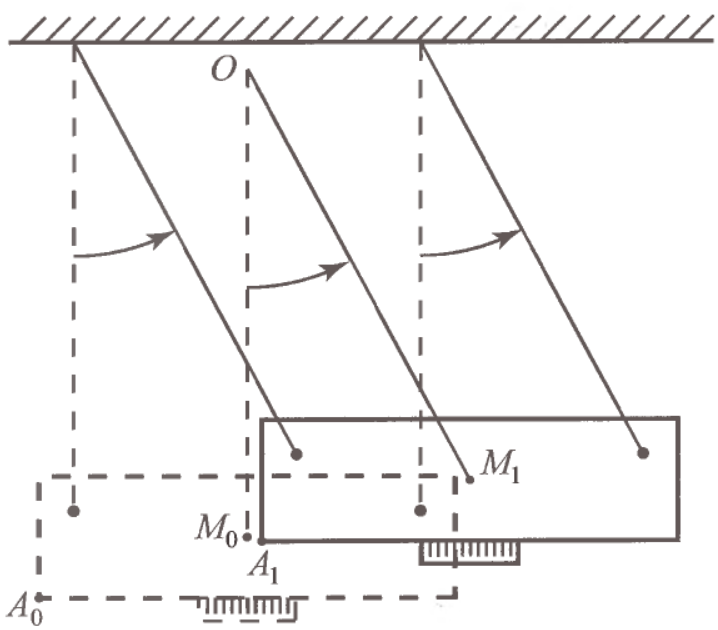
\includegraphics[width=0.6\linewidth]{pic_theory.png}

\label{fig:mpr}

\end{center}

Пренебрегая действием негоризонтальных внешних сил для системы пуля - цилиндр(сила тяжести и сила реакции опоры направлены вертикально), запишем ЗСИ.

\begin{equation}
	m u  = (M + m) V
\end{equation}

Здесь m - масса пули, M - масса цилиндра, u - скорость пули перед ударом, V - скорость цилиндра и пули после неупругого соударения.

Считая, что масса маятника много больше массы пули

\begin{equation}
	u  = \frac{M}{m} V
\end{equation}

В максимальной точке подъема вся кинетическая энергия маятника переходит в потенциальную. По ЗСЭ получу

\begin{equation}
	V^2 = 2 g h
\end{equation}

Считая угол отклонения от вертикали

\begin{equation}
	\phi = \frac{\Delta x}{L}
\end{equation}

получу высоту

\begin{equation}
	h = L (1 - \cos{\phi}) = 2 L sin^2 \frac{\phi}{2}
\end{equation}

Тогда итоговая формула для скорости


\[
\boxed{u = \frac{M}{m} \sqrt{\frac{g}{L}} \Delta x}
\]

\newpage

1) Изучу схему установки.

\begin{center}

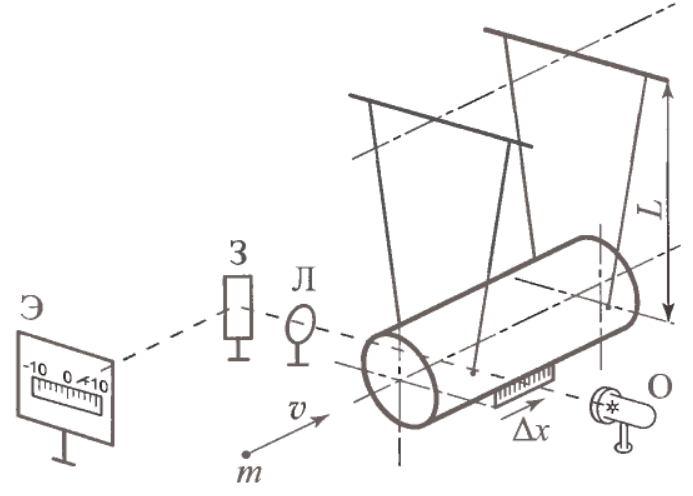
\includegraphics[width=0.6\linewidth]{pic_1.png}

\label{fig:mpr}

\end{center}

Перед началом работы внимательно изучу устройство баллистического ружья, чтобы не допустить критических ошибок при выполнении работы.


2) Использую аналитические весы для измерения масс пулек. Расположу каждую пулю в центре платформы для взвешивания, предварительно убедившить в том, что весы откалиброваны(арретированы).

Приведу сводную таблицу масс пулек

\begin{center}
\begin{tabular}[t]{|l|l|}

\hline
№ Пульки & Масса(г) \\
\hline
1 & 0.5030 \\
2 & 0.4958 \\
3 & 0.4981 \\
4 & 0.5080 \\
\hline
5 & 0.5081 \\
6 & 0.5011 \\
7 & 0.5087 \\
8 & 0.5082 \\
\hline
\end{tabular}
\end{center}

3) Длина подвеса

\begin{equation}
	L = (221.0 \pm 0.5)\text{ см}
\end{equation}

Вследствии неопределенности точки подвеса реальная неточность определения L может быть выше

4) Воспользуемся заранее откалиброванной системе(спасибо преподавателям)

5) Заведем ружье как положено. Влияние воздушной струи даже более незаметно, чем влияние воздужных потоков вследствии передвижения экспериментаторов.

6) Убедимся в пренебрежимости затуханий по результатам первого выстрела. Оценочная скорость затухания по изменению амплитуды за 20 колебаний:

\begin{equation}
	\delta_A = \frac{11.75 - 10.75}{20} = 0.05 \text{ мм} = 0.5 \% \ll 1
\end{equation}

Так что затуханием можно вполне пренебречь. За 10 колебаний амплитуда уменьшается в 10 раз меньше чем наполовину.

7) Перед каждым выстрелом остановлю колебания маятника. Затем произведу выстрелы. Поскольку затухание между двумя соседними колебаниями пренебрежимо мало, усредню несколько первых значений амплитуды, чтобы исключить случайную погрешность. Для точного измерения амплидуды с помощью компьютера произведу раскадровку и точно вычислю каждое отклонение.

Сделаю сводную таблицу по каждому выстрелу

\begin{center}
\begin{tabular}[t]{|l|l|l|l|}
\hline
№ Пульки & $x_{max}$, мм & $x_0$, мм & $\Delta x$, мм \\
\hline
1 & 10.3 & 1.6 & 11.9 \\
2 & 9.0 & 2.6 & 11.6 \\
3 & 8.8 & 3.4 & 12.2 \\
4 & 7.8 & 4.4 & 12.2 \\
\hline
\end{tabular}
\end{center}

\begin{equation}
	M = (2925 \pm 5) \text{ г}
\end{equation}

Используя формулу

\begin{equation}
	u = \frac{M}{m}\sqrt{\frac{g}{L}} \Delta x
\end{equation}

рассчитаю соответствующие $u_i$ и занесу их в сводную таблицу по параметрам каждого выстрела

\begin{center}
\begin{tabular}[t]{|l|l|l|l|}
\hline
№ Пульки & m, г & $\Delta x$, мм & u, м/с \\
\hline
1 & 0.5030 & 11.9 & $(146 \pm 4)$ \\
2 & 0.4958 & 11.6 & $(144 \pm 4)$ \\
3 & 0.4981 & 12.2 & $(151 \pm 4)$ \\
4 & 0.5080 & 12.2 & $(148 \pm 4)$ \\
\hline
\end{tabular}
\end{center}

8) Для определения погрешности u продифференцирую соответствующую формулу

\begin{equation}
	\epsilon_u = \epsilon_M + \epsilon_m + \frac{\epsilon_g + \epsilon_L}{2} + \epsilon_{\Delta x} = \frac{5}{2925} + \frac{0.0001}{0.5} + \frac{0.25}{12} = 2.5\%
\end{equation}

Как видно, основной вклад вносит именно погрешность измерения амплитуды колебаний маятника

Класс точности аналитических весов обеспечивает большую, чем последняя цифра, точность, поэтому в расчет возьму последнюю. Ускорение свободного падения в Москве приму за $(9.815 \pm 0.001) \text{ m}/s^2$

9) Среднее значение скорости найду по формуле

\begin{equation}
\overline{u} = \sum^N_{i=1} u_i = 147 \text{ м/с}
\end{equation}

Среднеквадратичные отклонения и ошибка вычисляются следующим образом

\begin{equation}
\left\{
\begin{aligned}
\sigma_{\text{откл}} = \sqrt{\frac{1}{N} \sum^N_{i=1} \left( n_i - \overline{n} \right)^2} = 3 \text{ м/с} \\	
\sigma_{\text{ошиб}} = \sqrt{\frac{1}{N (N - 1)} \sum^N_{i=1} \left( n_i - \overline{n} \right)^2} = 1.5 \text{ м/с}
\end{aligned}
\right.
\end{equation}


Суммарная ошибка

\begin{equation}
	\sigma_0 = \sqrt{\sigma_{\text{ошиб}} ^ 2 + \left( \epsilon_u \cdot u \right) ^2} = 4 \text{ m}/s
\end{equation}

Итого

\begin{equation}
	u = (147 \pm 4) \text{ m}/s
\end{equation}


Как видно, случайная погрешность довольно мала. Погрешность метода изменений получается больше. Разумным был бы ответ, что это исключительно ошибка метода измерений и скорость пули действительно постоянна при каждом выстреле. Но дополнительно были произведены замеры скоростей пули специализированным прибором, и они дали совпадающие с 3 и 4 измерением результаты. Как следствие, следовало бы предположить, что скорость пули действительно меняется при различных выстрелах, причем сопоставимо с уже измеренными погрешностями.

В итоге разброс связан как с ошибками опыта, так и с различием скоростей от выстрела к выстрелу, причем в равной степени.

\newpage
\begin{bfseries}
	Часть 2. "Вращательный" маятник.
\end{bfseries}

Выведу основные формулы

Считая удар пули неупругим, для определения скорости пули воспользуюсь ЗСМИ

\begin{equation}
	m u r = I \Omega
\end{equation}

Все величины указаны на схеме установки

Пренебрегая потерями энергии на трение, запишу ЗСЭ

\begin{equation}
	k \frac{\phi^2}{2} = I \frac{\Omega^2}{2}
\end{equation}

k - модуль кручения проволки, $\phi$ - максимальный угол поворота маятника

Получим в итоге

\[
\boxed{u = \phi \frac{\sqrt{k I}}{m r}}
\]

Из схемы следует, что т.к. угол малый, то

\begin{equation}
	\phi \approx \frac{x}{2 d}
\end{equation}

Рассмотрю $T_1$ - период колебаний без грузов M, $T_2$ - с ними

\begin{equation}
	T_1 = 2 \pi \sqrt{\frac{I}{k}}
\end{equation}

\begin{equation}
	T_2 = 2 \pi \sqrt{\frac{I - 2 M R^2}{k}}
\end{equation}

Наконец

\[
\boxed{\sqrt{k I} = \frac{4 \pi M R^2 T_1}{T_1^2 - T_2^2}}
\]

\newpage

1) Изучу схему установки.

\begin{center}

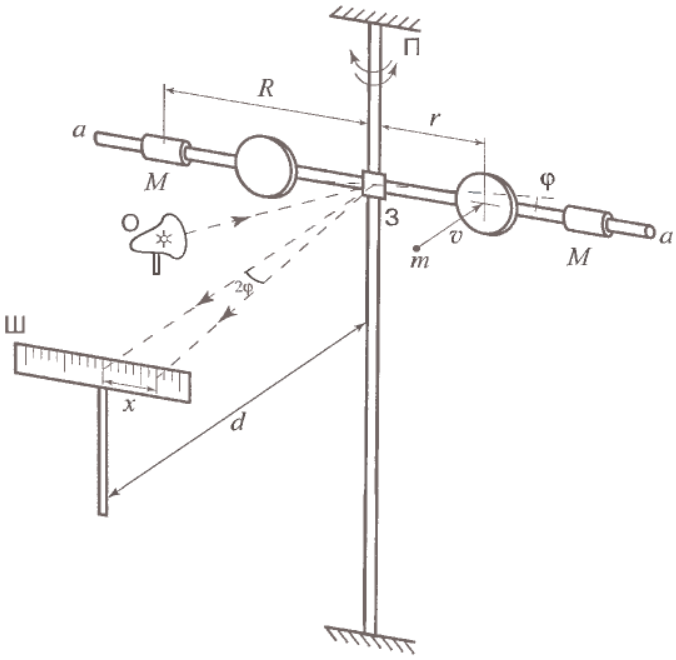
\includegraphics[width=0.6\linewidth]{pic_2.png}

\label{fig:mpr}

\end{center}

2) Смотри часть 1

3) Приведу табличку с этими расстояниями

\begin{center}
\begin{tabular}[t]{|l|l|l|l|}
\hline
d, см & R, см & r, см \\
\hline
$(50.0 \pm 0.1)$ & $(33.7 \pm 0.1)$ & $(23.1 \pm 0.1)$ \\
\hline
\end{tabular}
\end{center}

4) В процессе опыта иногда придется перенастраивать систему, смещая нормировку местоположением тени нити на шкале(желательно держать её около нуля)

5 )Аналогично части 1 воздущным потоком можно пренебрегать.

6) Убедимся в пренебрежимости затуханий по результатам первого выстрела. Оценочная скорость затухания по изменению амплитуды за 20 колебаний:

\begin{equation}
	\delta_A = \frac{18 - 16}{10} = 0.2 \text{ см} = 1 \% \ll 1
\end{equation}

Затухание несильно больше соответствующего в части 1, поэтому им также можно спокойно пренебречь в рамках производимых измерений.

7) Для точного вычисления периодов применю метод рядов, то есть замер 10 подряд идущих периодов колебаний с последующим вычислением одного.

Результаты измерений приведу вместе

\begin{equation}
	\left\{
		\begin{aligned}
			T_1 = (13.7 \pm 0.05) \text{ сек} \\
			T_2 = (17.8 \pm 0.05) \text{ сек}
		\end{aligned}
	\right.
\end{equation}

Погрешность написана с оценкой времени реакции экспериментатора, а также цены деления шкалы.

\begin{equation}
	M = 714.0 \text{ г}
\end{equation}

Расчитаю инерционный параметр

\begin{equation}
	\sqrt{k I} = \frac{4 \pi M R^2 T_1}{T_1^2 - T_2^2} = 0.108 \pm 0.002 \text{ }\frac{\text{кг} \cdot \text{м}^2}{\text{с}}
\end{equation}

Погрешность я вычислил методом границы диапазона

\begin{equation}
	max(\sqrt{k I}) = \frac{4 \pi M (R + \Delta R)^2 (T_1 + \Delta T_1)}{T_1^2 - T_2^2} = 0.110 \text{ }\frac{\text{кг} \cdot \text{м}^2}{\text{с}}
\end{equation}

Тогда $\sigma_{sqrt} \approx 0.110 - 0.108 = 0.002$

8) Проделаю подобную части 1 процедуру.

Сделаю сводную таблицу по каждому выстрелу.

\begin{center}
\begin{tabular}[t]{|l|l|l|l|}
\hline
№ Пульки & $x_{max}$, cм & $x_{min}$, cм & $\Delta x$, cм \\
\hline
5 & 19.5 & -13.6 & 16.6 \\
6 & 17.2 & -15.0 & 16.1 \\
7 & 22.9 & -11.6 & 17.3 \\
8 & 23.3 & -11.6 & 17.5 \\
\hline
\end{tabular}
\end{center}

Итоговая формула для расчета скорости пули

\begin{equation}
	u = \frac{\sqrt{k I} \Delta x}{2 m r d}
\end{equation}

Приведу итоговую таблицу

\begin{center}
\begin{tabular}[t]{|l|l|l|l|}
\hline
№ Пульки & m, г & $\Delta x$, см & u, м/с \\
\hline
1 & 0.5081 & 16.6 & $(153 \pm 4)$ \\
2 & 0.5011 & 16.1 & $(150 \pm 4)$ \\
3 & 0.5087 & 17.3 & $(159 \pm 4)$ \\
4 & 0.5082 & 17.5 & $(161 \pm 4)$ \\
\hline
\end{tabular}
\end{center}

9) Оценю погрешность определения $\Delta x$. По порядку она равна диаметру тени, создаваемой ниткой, т.е. 4 мм.

Для определения погрешности u продифференцирую соответствующую формулу

\begin{equation}
	\epsilon_u = \epsilon_{sqrt} + \epsilon_{\Delta x} + \epsilon_m + \epsilon_{r} + \epsilon_{d} = \frac{0.1}{50} + \frac{0.0001}{0.5} + \frac{0.1}{20.4} + \frac{0.1}{50} + \frac{0.4}{16} = 5\%
\end{equation}

Как видно, основной вклад вносит именно погрешность измерения амплитуды колебаний маятника. Расчет выполнил со значениями на основе части 1.

9) Среднее значение скорости

\begin{equation}
	\overline{u} = 156 \text{ m}/s^2
\end{equation}

Среднеквадратичные отклонения и ошибка

\begin{equation}
\left\{
\begin{aligned}
\sigma_{\text{откл}} \approx 4 \text{ m}/s \\	
\sigma_{\text{ошиб}} \approx 3 \text{ m}/s
\end{aligned}
\right.
\end{equation}

Суммарная ошибка

\begin{equation}
	\sigma_0 =  8 \text{ m}/s
\end{equation}

Итого

\begin{equation}
	u = (156 \pm 8) \text{ m}/s
\end{equation}

Как видно, случайная погрешность довольно мала. Погрешность метода изменений получается больше в 2 раза. Поэтому в рамках этой серии замеров можно сказать, что разброс связан с погрешностями измерений.

\newpage
\begin{bfseries}
	Вывод.
\end{bfseries}

Замеры скоростей для обоих установок довольно схожи(в рамках погрешностей). В совокупности всех замеров можно сказать, что результаты первого эксперимента более верные. Неточность же второго эксперимента можно объяснить сложностью установки, а значит неучтенными систематическими погрешностями.

Поэтому следует считать, что 

\begin{equation}
	u = (147 \pm 4) \text{ m}/s
\end{equation}

\end{problem}
\end{document}